
\documentclass[12pt]{article}

% Layout.
\usepackage[top=1in, bottom=0.75in, left=1in, right=1in, headheight=1in, headsep=6pt]{geometry}

% Fonts.
\usepackage{mathptmx}
\usepackage[scaled=0.86]{helvet}
\renewcommand{\emph}[1]{\textsf{\textbf{#1}}}

% TiKZ.
\usepackage{tikz, pgfplots}
\usetikzlibrary{calc}
\pgfplotsset{compat = newest}
 
\pgfplotsset{my style/.append style={axis x line=middle, axis y line=
middle, xlabel={$x$}, ylabel={$y$}, axis equal
}}

% Misc packages.
\usepackage{amsmath,amssymb,latexsym}
\usepackage{graphicx}
\usepackage{array}
\usepackage{xcolor}
\usepackage{multicol}

% Commands to set various header/footer components.
\makeatletter
\def\doctitle#1{\gdef\@doctitle{#1}}
\doctitle{Use {\tt\textbackslash doctitle\{MY LABEL\}}.}
\def\docdate#1{\gdef\@docdate{#1}}
\docdate{Use {\tt\textbackslash docdate\{MY DATE\}}.}
\def\doccourse#1{\gdef\@doccourse{#1}}
\let\@doccourse\@empty
\def\docscoring#1{\gdef\@docscoring{#1}}
\let\@docscoring\@empty
\def\docversion#1{\gdef\@docversion{#1}}
\let\@docversion\@empty
\makeatother

% Headers and footers layout.
\makeatletter
\usepackage{fancyhdr}
\pagestyle{fancy}
\fancyhf{} % Clears all headers/footers.
\lhead{\baselineskip 30pt
%\emph{\@doctitle\hfill\@docdate}
\emph{\@docdate\hfill\@doctitle}
\ifnum \value{page} > 1\relax\else\\
\emph{Name: \rule{3.5in}{1pt}\hfill \@docscoring}\fi}
\rfoot{\emph{\@docversion}}
\lfoot{\emph{\@doccourse}}
\cfoot{\emph{\thepage}}
\renewcommand{\headrulewidth}{0pt}%
\makeatother

% Paragraph spacing
\parindent 0pt
\parskip 6pt plus 1pt

% A problem is a section-like command. Use \problem{5} to
% start a problem worth 5 points.
\newcounter{probcount}
\newcounter{subprobcount}
\setcounter{probcount}{0}
\newcommand{\problem}[1]{%
\par
\addvspace{4pt}%
\setcounter{subprobcount}{0}%
\stepcounter{probcount}%
\makebox[0pt][r]{\emph{\arabic{probcount}.}\hskip1ex}\emph{[#1 points]}\hskip1ex}
\newcommand{\thesubproblem}{\emph{\alph{subprobcount}.}}

% Subproblems are an enumerate-like environment with a consistent
% numbering scheme. 
% Use \begin{subproblems}\item...\item...\end{subproblems}
\newenvironment{subproblems}{%
\begin{enumerate}%
\setcounter{enumi}{\value{subprobcount}}%
\renewcommand{\theenumi}{\emph{\alph{enumi}}}}%
{\setcounter{subprobcount}{\value{enumi}}\end{enumerate}}

% Blanks for answers in normal and math mode.
\newcommand{\blank}[1]{\rule{#1}{0.75pt}}
\newcommand{\mblank}[1]{\underline{\hspace{#1}}}
\def\emptybox(#1,#2){\framebox{\parbox[c][#2]{#1}{\rule{0pt}{0pt}}}}

% Misc.
\renewcommand{\d}{\displaystyle}
\newcommand{\ds}{\displaystyle}
\def\bc{\begin{center}}
\def\ec{\end{center}}
\def\be{\begin{enumerate}}
\def\ee{\end{enumerate}}


\doctitle{Math 251: Quiz 4}
\docdate{Sept 22, 2022}
\doccourse{UAF Calculus I}
\docversion{v-1}
\docscoring{\blank{0.8in} / 25}
\begin{document}

There are 25 points possible on this quiz. No aids (book, calculator, etc.)
are permitted.  {\bf Show all work for full credit.}

\problem{2} State the definition of $f'(x),$ the derivative of the function $f(x).$\\
\vspace{1in}
\problem{8} \textbf{Use the definition} (above) to find the derivative $f'(x)$ when $f(x)=\frac{5}{x+1}.$
\vfill
\newpage
\problem{3} Use the Quotient Rule to find $f'(x)$ if $f(x)=\frac{\sin(x)}{x^2+1}.$ (You do not need to simplify your answer.)
\vfill
\problem{6} Find the derivative for each function below. Simplify your answer. 
\begin{subproblems}
	\item $y=2x^{4.1}- x +\pi^2$
	\vfill
	\item $y=7x\cos(x)$
	\vfill
\end{subproblems}

\problem{6} Assume $C(q)$ is the cost, in dollars, of manufacturing $q$ widgets. 
\begin{subproblems}
\item Using a complete sentence (or sentences), interpret the meaning of $C(50)=1120.$
\vfill
\item What are the units of $C'(q)$?
\vfill
\item Using a complete sentence (or sentences), interpret the meaning of $C'(50)=15.$
\vfill
\end{subproblems}

\end{document}

\newpage
\problem{8} Use the graph of $f(x)$ (below) to answer the questions. 

\begin{center}
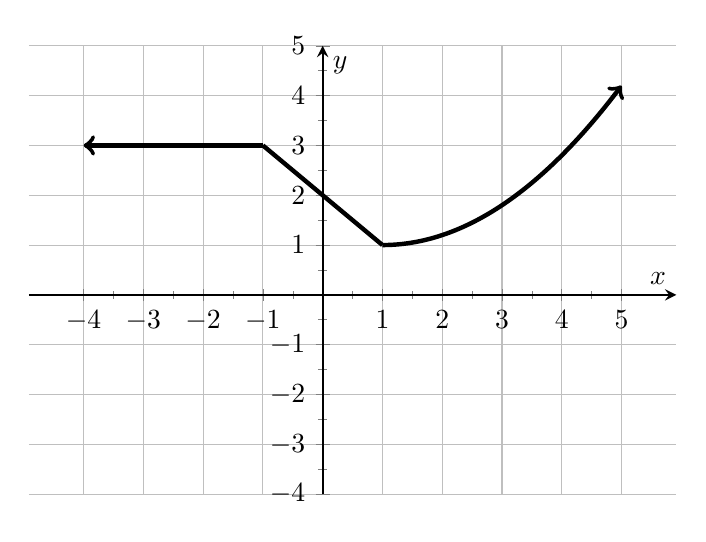
\begin{tikzpicture}
%cubic
\begin{axis}[xscale=1.2, thick, my style, xtick={-4,-3,-2,...,3,4,5}, ytick={-4,-3,...,5},xmin=-4, xmax=5, ymin=-4, ymax=5, minor y tick num=1, minor x tick num=1, 
mark size=3.0pt, grid = major]
\addplot[ultra thick, <-,domain=-4:-1, samples=100]{3};
\addplot[ultra thick,domain=-1:1, samples=100]{2-x};
\addplot[ultra thick, ->,domain=1:5, samples=100]{1+(0.2)*(x-1)*(x-1)};
\end{axis}
\end{tikzpicture}\end{center}
\vfill
\begin{subproblems}
\item Evaluate the derivatives below or state that they do not exist.\\
$f'(-3)=$ \hfill $f'(-1)$ \hfill  $f'()$ \hfill\quad

\item Sketch $f'$
\end{subproblems}

\problem{3} Find the derivative $H(x)=\sqrt{2}-x+4\sin(x)+\frac{2}{3x}$. You do not need to simplify.
\vspace{1in}



\end{document}